\documentclass[tikz,border=10pt]{standalone}
\usepackage{tikz}
\usetikzlibrary{shapes.geometric, arrows.meta, positioning, calc, fit, backgrounds}
\usepackage{amsmath,amssymb}
\usepackage{xcolor}

% Unified Academic Color Palette
\definecolor{cInput}{RGB}{235, 248, 255}
\definecolor{bInput}{RGB}{49, 130, 206}

\definecolor{cTrans}{RGB}{240, 249, 255}
\definecolor{bTrans}{RGB}{43, 108, 176}

\definecolor{cGCN}{RGB}{230, 255, 250}
\definecolor{bGCN}{RGB}{49, 151, 149}

\definecolor{cRecurr}{RGB}{250, 245, 255}
\definecolor{bRecurr}{RGB}{128, 90, 213}

\definecolor{cHead}{RGB}{255, 245, 245}
\definecolor{bHead}{RGB}{229, 62, 62}

\definecolor{cFusion}{RGB}{254, 252, 191}
\definecolor{bFusion}{RGB}{214, 158, 46}

\definecolor{cGray}{RGB}{247, 250, 252}
\definecolor{bGray}{RGB}{160, 174, 192}

\definecolor{tDark}{RGB}{26, 32, 44}
\definecolor{tMuted}{RGB}{74, 85, 104}

\begin{document}
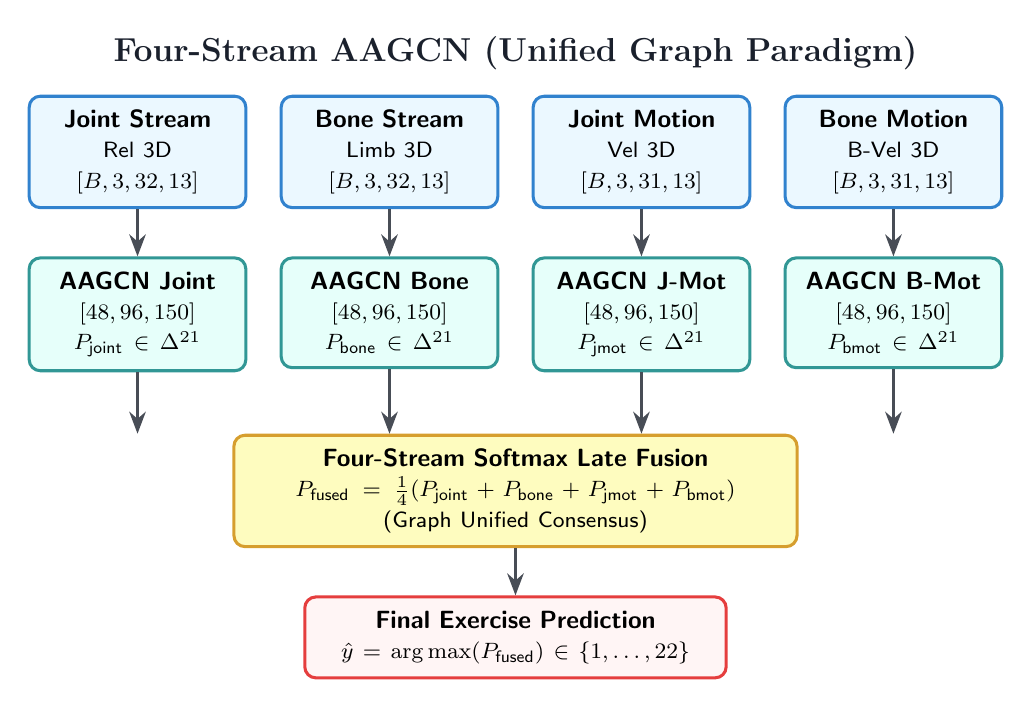
\begin{tikzpicture}[
    font=\sffamily\small,
    >=Stealth,
    node distance=0.6cm,
    block/.style={
        draw=#1,
        line width=1.1pt,
        rounded corners=4pt,
        align=center,
        inner sep=5pt
    },
    arrow/.style={->, line width=1.1pt, color=tDark!80}
]

\node[font=\bfseries\large, text=tDark] (title) at (5.7, 1.25) {Four-Stream AAGCN (Unified Graph Paradigm)};

\node[block=bInput, fill=cInput, text width=2.4cm] (in1) at (0.9, 0) {
    \textbf{Joint Stream}\\
    {\footnotesize Rel 3D $[B,3,32,13]$}
};
\node[block=bGCN, fill=cGCN, text width=2.4cm, below=of in1] (back1) {
    \textbf{AAGCN Joint}\\
    {\footnotesize $[48, 96, 150]$}\\
    {\footnotesize $P_{\text{joint}} \in \Delta^{21}$}
};

\node[block=bInput, fill=cInput, text width=2.4cm] (in2) at (4.1, 0) {
    \textbf{Bone Stream}\\
    {\footnotesize Limb 3D $[B,3,32,13]$}
};
\node[block=bGCN, fill=cGCN, text width=2.4cm, below=of in2] (back2) {
    \textbf{AAGCN Bone}\\
    {\footnotesize $[48, 96, 150]$}\\
    {\footnotesize $P_{\text{bone}} \in \Delta^{21}$}
};

\node[block=bInput, fill=cInput, text width=2.4cm] (in3) at (7.3, 0) {
    \textbf{Joint Motion}\\
    {\footnotesize Vel 3D $[B,3,31,13]$}
};
\node[block=bGCN, fill=cGCN, text width=2.4cm, below=of in3] (back3) {
    \textbf{AAGCN J-Mot}\\
    {\footnotesize $[48, 96, 150]$}\\
    {\footnotesize $P_{\text{jmot}} \in \Delta^{21}$}
};

\node[block=bInput, fill=cInput, text width=2.4cm] (in4) at (10.5, 0) {
    \textbf{Bone Motion}\\
    {\footnotesize B-Vel 3D $[B,3,31,13]$}
};
\node[block=bGCN, fill=cGCN, text width=2.4cm, below=of in4] (back4) {
    \textbf{AAGCN B-Mot}\\
    {\footnotesize $[48, 96, 150]$}\\
    {\footnotesize $P_{\text{bmot}} \in \Delta^{21}$}
};

\draw[arrow] (in1) -- (back1);
\draw[arrow] (in2) -- (back2);
\draw[arrow] (in3) -- (back3);
\draw[arrow] (in4) -- (back4);

% Fusion
\node[block=bFusion, fill=cFusion, text width=6.8cm, below=0.8cm of $(back2.south)!0.5!(back3.south)$] (fuse) {
    \textbf{Four-Stream Softmax Late Fusion}\\
    {\footnotesize $P_{\text{fused}} = \frac{1}{4}(P_{\text{joint}} + P_{\text{bone}} + P_{\text{jmot}} + P_{\text{bmot}})$}\\
    {\footnotesize (Graph Unified Consensus)}
};

\node[block=bHead, fill=cHead, text width=5.0cm, below=of fuse] (pred) {
    \textbf{Final Exercise Prediction}\\
    {\footnotesize $\hat{y} = \arg\max(P_{\text{fused}}) \in \{1, \dots, 22\}$}
};

\draw[arrow] (back1.south) -- (fuse.north -| back1.south);
\draw[arrow] (back2.south) -- (fuse.north -| back2.south);
\draw[arrow] (back3.south) -- (fuse.north -| back3.south);
\draw[arrow] (back4.south) -- (fuse.north -| back4.south);
\draw[arrow] (fuse) -- (pred);

\end{tikzpicture}
\end{document}
